% CVPR 2022 Paper Template
% based on the CVPR template provided by Ming-Ming Cheng (https://github.com/MCG-NKU/CVPR_Template)
% modified and extended by Stefan Roth (stefan.roth@NOSPAMtu-darmstadt.de)

\documentclass[10pt,twocolumn,letterpaper]{article}

%%%%%%%%% PAPER TYPE  - PLEASE UPDATE FOR FINAL VERSION %%%%%%%%%
%\usepackage[review]{cvpr}      % To produce the REVIEW version
%\usepackage{cvpr}              % To produce the CAMERA-READY version
\usepackage[pagenumbers]{cvpr} % To force page numbers, e.g. for an arXiv version

% Include other packages here, before hyperref.
\usepackage{graphicx}
\usepackage{amsmath}
\usepackage{amssymb}
\usepackage{booktabs}
\usepackage{float}
\usepackage{arydshln}
\usepackage{enumitem}


% It is strongly recommended to use hyperref, especially for the review version.
% hyperref with option pagebackref eases the reviewers' job.
% Please disable hyperref *only* if you encounter grave issues, e.g. with the
% file validation for the camera-ready version.
%
% If you comment hyperref and then uncomment it, you should delete
% ReviewTempalte.aux before re-running LaTeX.
% (Or just hit 'q' on the first LaTeX run, let it finish, and you
%  should be clear).
\usepackage[pagebackref,breaklinks,colorlinks]{hyperref}


% Support for easy cross-referencing
\usepackage[capitalize]{cleveref}
\crefname{section}{Sec.}{Secs.}
\Crefname{section}{Section}{Sections}
\Crefname{table}{Table}{Tables}
\crefname{table}{Tab.}{Tabs.}

\raggedbottom
\begin{document}

%%%%%%%%% TITLE - PLEASE UPDATE %%%%%%%%%
\title{DLP Lab4: Conditional VAE for Video Prediction}

\author{Yi-Hsiang Ho, 111550106
% For a paper whose authors are all at the same institution,
% omit the following lines up until the closing ``}''.
% Additional authors and addresses can be added with ``\and'',
% just like the second author.
% To save space, use either the email address or home page, not both
% \and
% Second Author\\
% Institution2\\
% First line of institution2 address\\
% {\tt\small secondauthor@i2.org}
}
\maketitle

%%%%%%%%% BODY TEXT %%%%%%%%%

\section{Introduction}
\label{sec:lab4_intro}

In this lab, I worked on pose-conditioned video prediction: given the first RGB
frame and a pose sequence, the model predicts future RGB frames in an
autoregressive way. Since long-horizon rollout easily accumulates errors, the
model needs both good reconstruction and stable training.

Instead of spending most effort on designing a brand-new architecture, this
assignment is mainly about \,\emph{making the provided CVAE training reliable and
high-performing}. In practice, my final score is dominated by training tricks
and schedules. The main parts I focused on are:
\begin{itemize}[itemsep=1pt]
  \item \textbf{Teacher forcing schedule}: start with a moderate ratio and decay
    after a few epochs to help the model transition to self-conditioned rollout.
  \item \textbf{KL annealing}: warm up the KL weight (monotonic works best in my
    runs) to avoid strong regularization too early.
  \item \textbf{Data sampling tricks}: enable shuffling and use a sliding window
    to increase temporal diversity per epoch.
  \item \textbf{Inference trick}: use Monte Carlo averaging (multiple latent
    samples) to reduce variance in predictions.
\end{itemize}

\section{Implementation Details}
\label{sec:lab4_impl}

\subsection{Code Structure and Data Pipeline}

I mainly worked with four parts in the provided codebase: (1) the training
script, (2) the testing/inference script, (3) the dataloader, and (4) the model
modules (encoders, latent predictor, and decoder).

In the dataloader (\verb|Dataset_Dance|), frames are sorted by index and
organized into sequences. Specifically, training mode uses sliding windows with
configurable \verb|stride| for better temporal coverage.

In my experiments, I found that enabling training shuffle and using sliding
windows can give more diverse temporal windows per epoch, which helps
the model generalize better during autoregressive rollout.

\subsection{Training and Testing Protocol}
\label{sec:training_testing}

During training, the loop in \verb|training_stage()| iterates over epochs and
mini-batches (as shown in \cref{fig:impl_training_stage}). In each epoch, the teacher forcing ratio (tfr) and KL weight
$\beta$ are updated (details are discussed in the next few sections).

\begin{figure}[H]
  \centering
  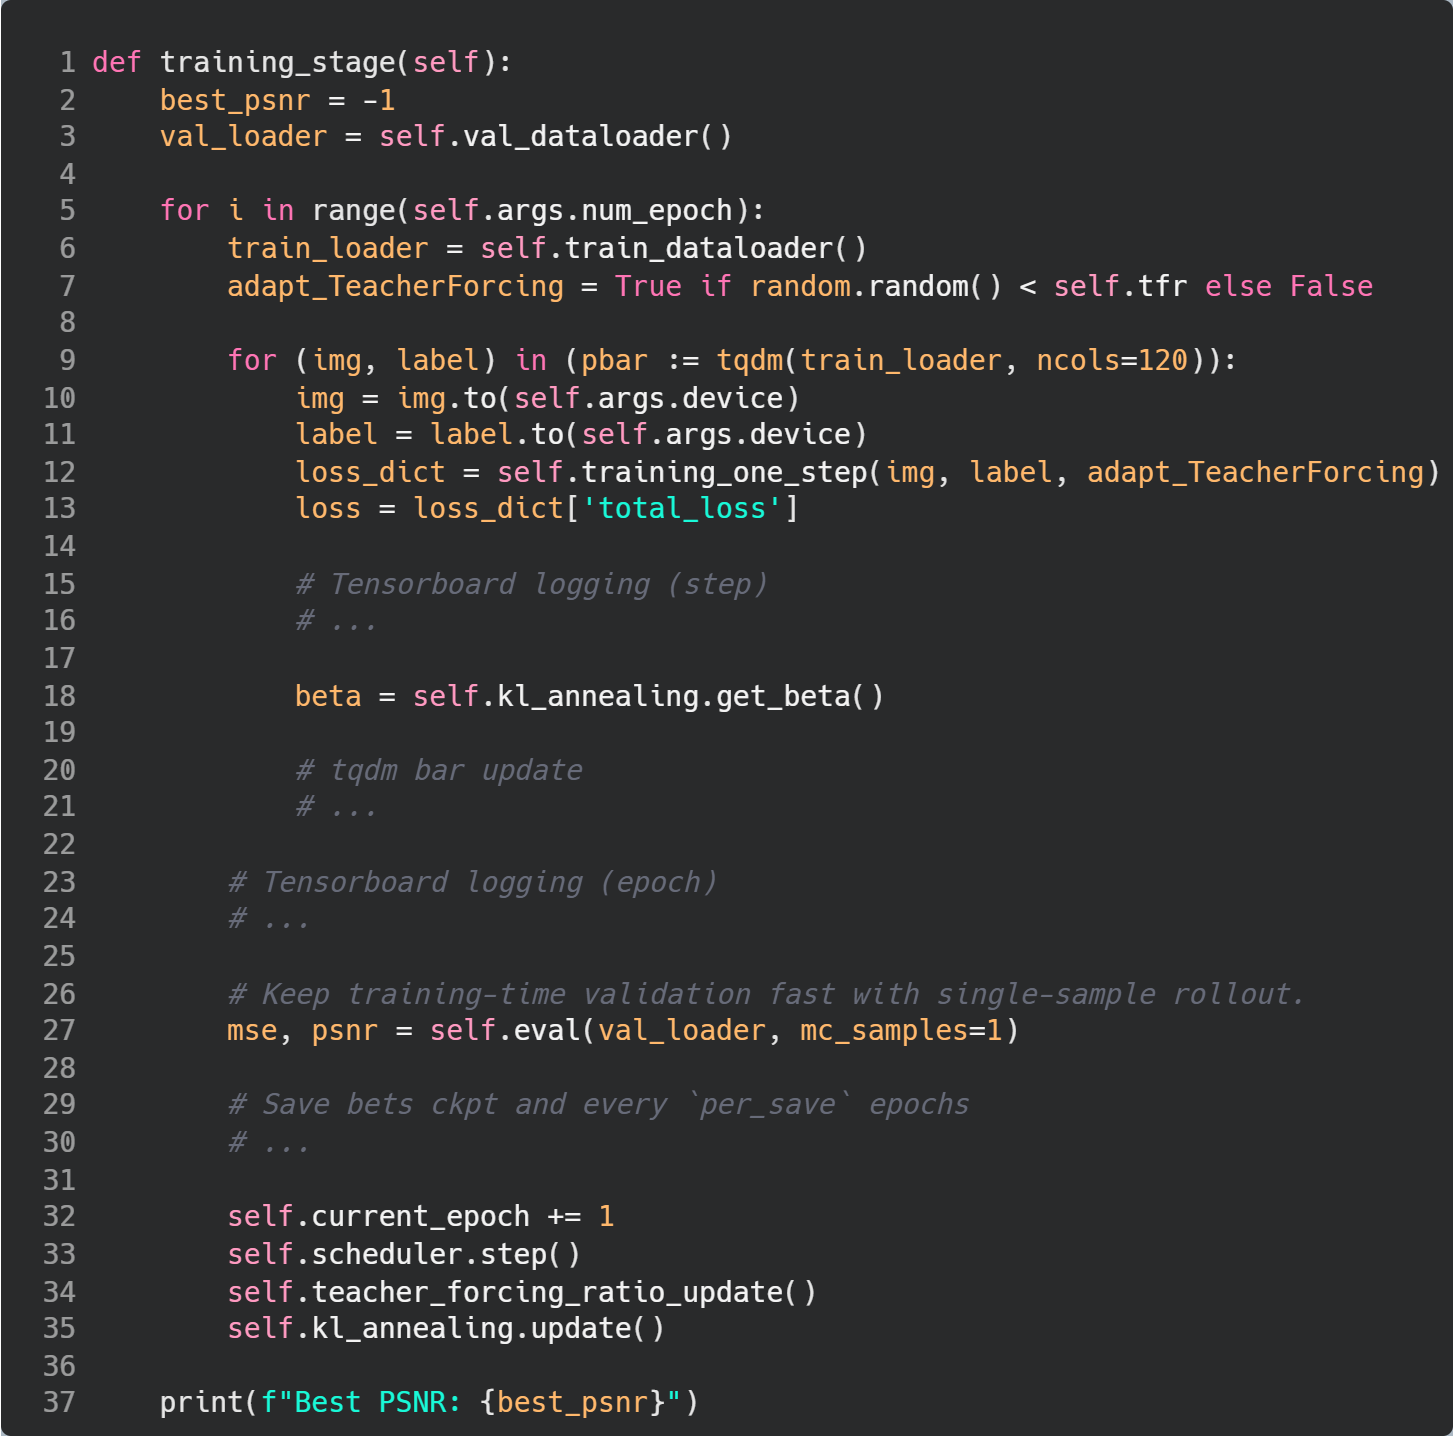
\includegraphics[width=\linewidth]{assets/impl-training_stage.png}
  \caption{\textbf{Training stage}: epoch loop, batch loop, and per-epoch updates.}
  \label{fig:impl_training_stage}
\end{figure}

In each batch, \verb|training_one_step()| executes these steps:
\begin{itemize}[itemsep=0pt]
  \item \textbf{Encode all frames/poses}.
  \item \textbf{Roll out over time}: for each timestep $t$, predict latent
    $z_t$ from encoder (\verb|Gaussian_Predictor|) using encoded image/label
    features.
  \item \textbf{Teacher forcing decision}: for $t>0$, the previous input frame is
  either the ground-truth frame $x_{t-1}$ or the previous prediction
  $\hat{x}_{t-1}$ (detached). With per-epoch teacher forcing, the decision is
  fixed for the whole epoch; with scheduled sampling, it is sampled per frame.
  \item \textbf{Decode next frame}: fuse (previous-frame feature, label feature,
  and $z_t$) with \verb|Decoder_Fusion|, then generate RGB with
  \verb|Generator| and \verb|sigmoid|.
\end{itemize}
I include the corresponding code structure in \cref{fig:impl_training_one_step}
for reference.

\begin{figure}[H]
  \centering
  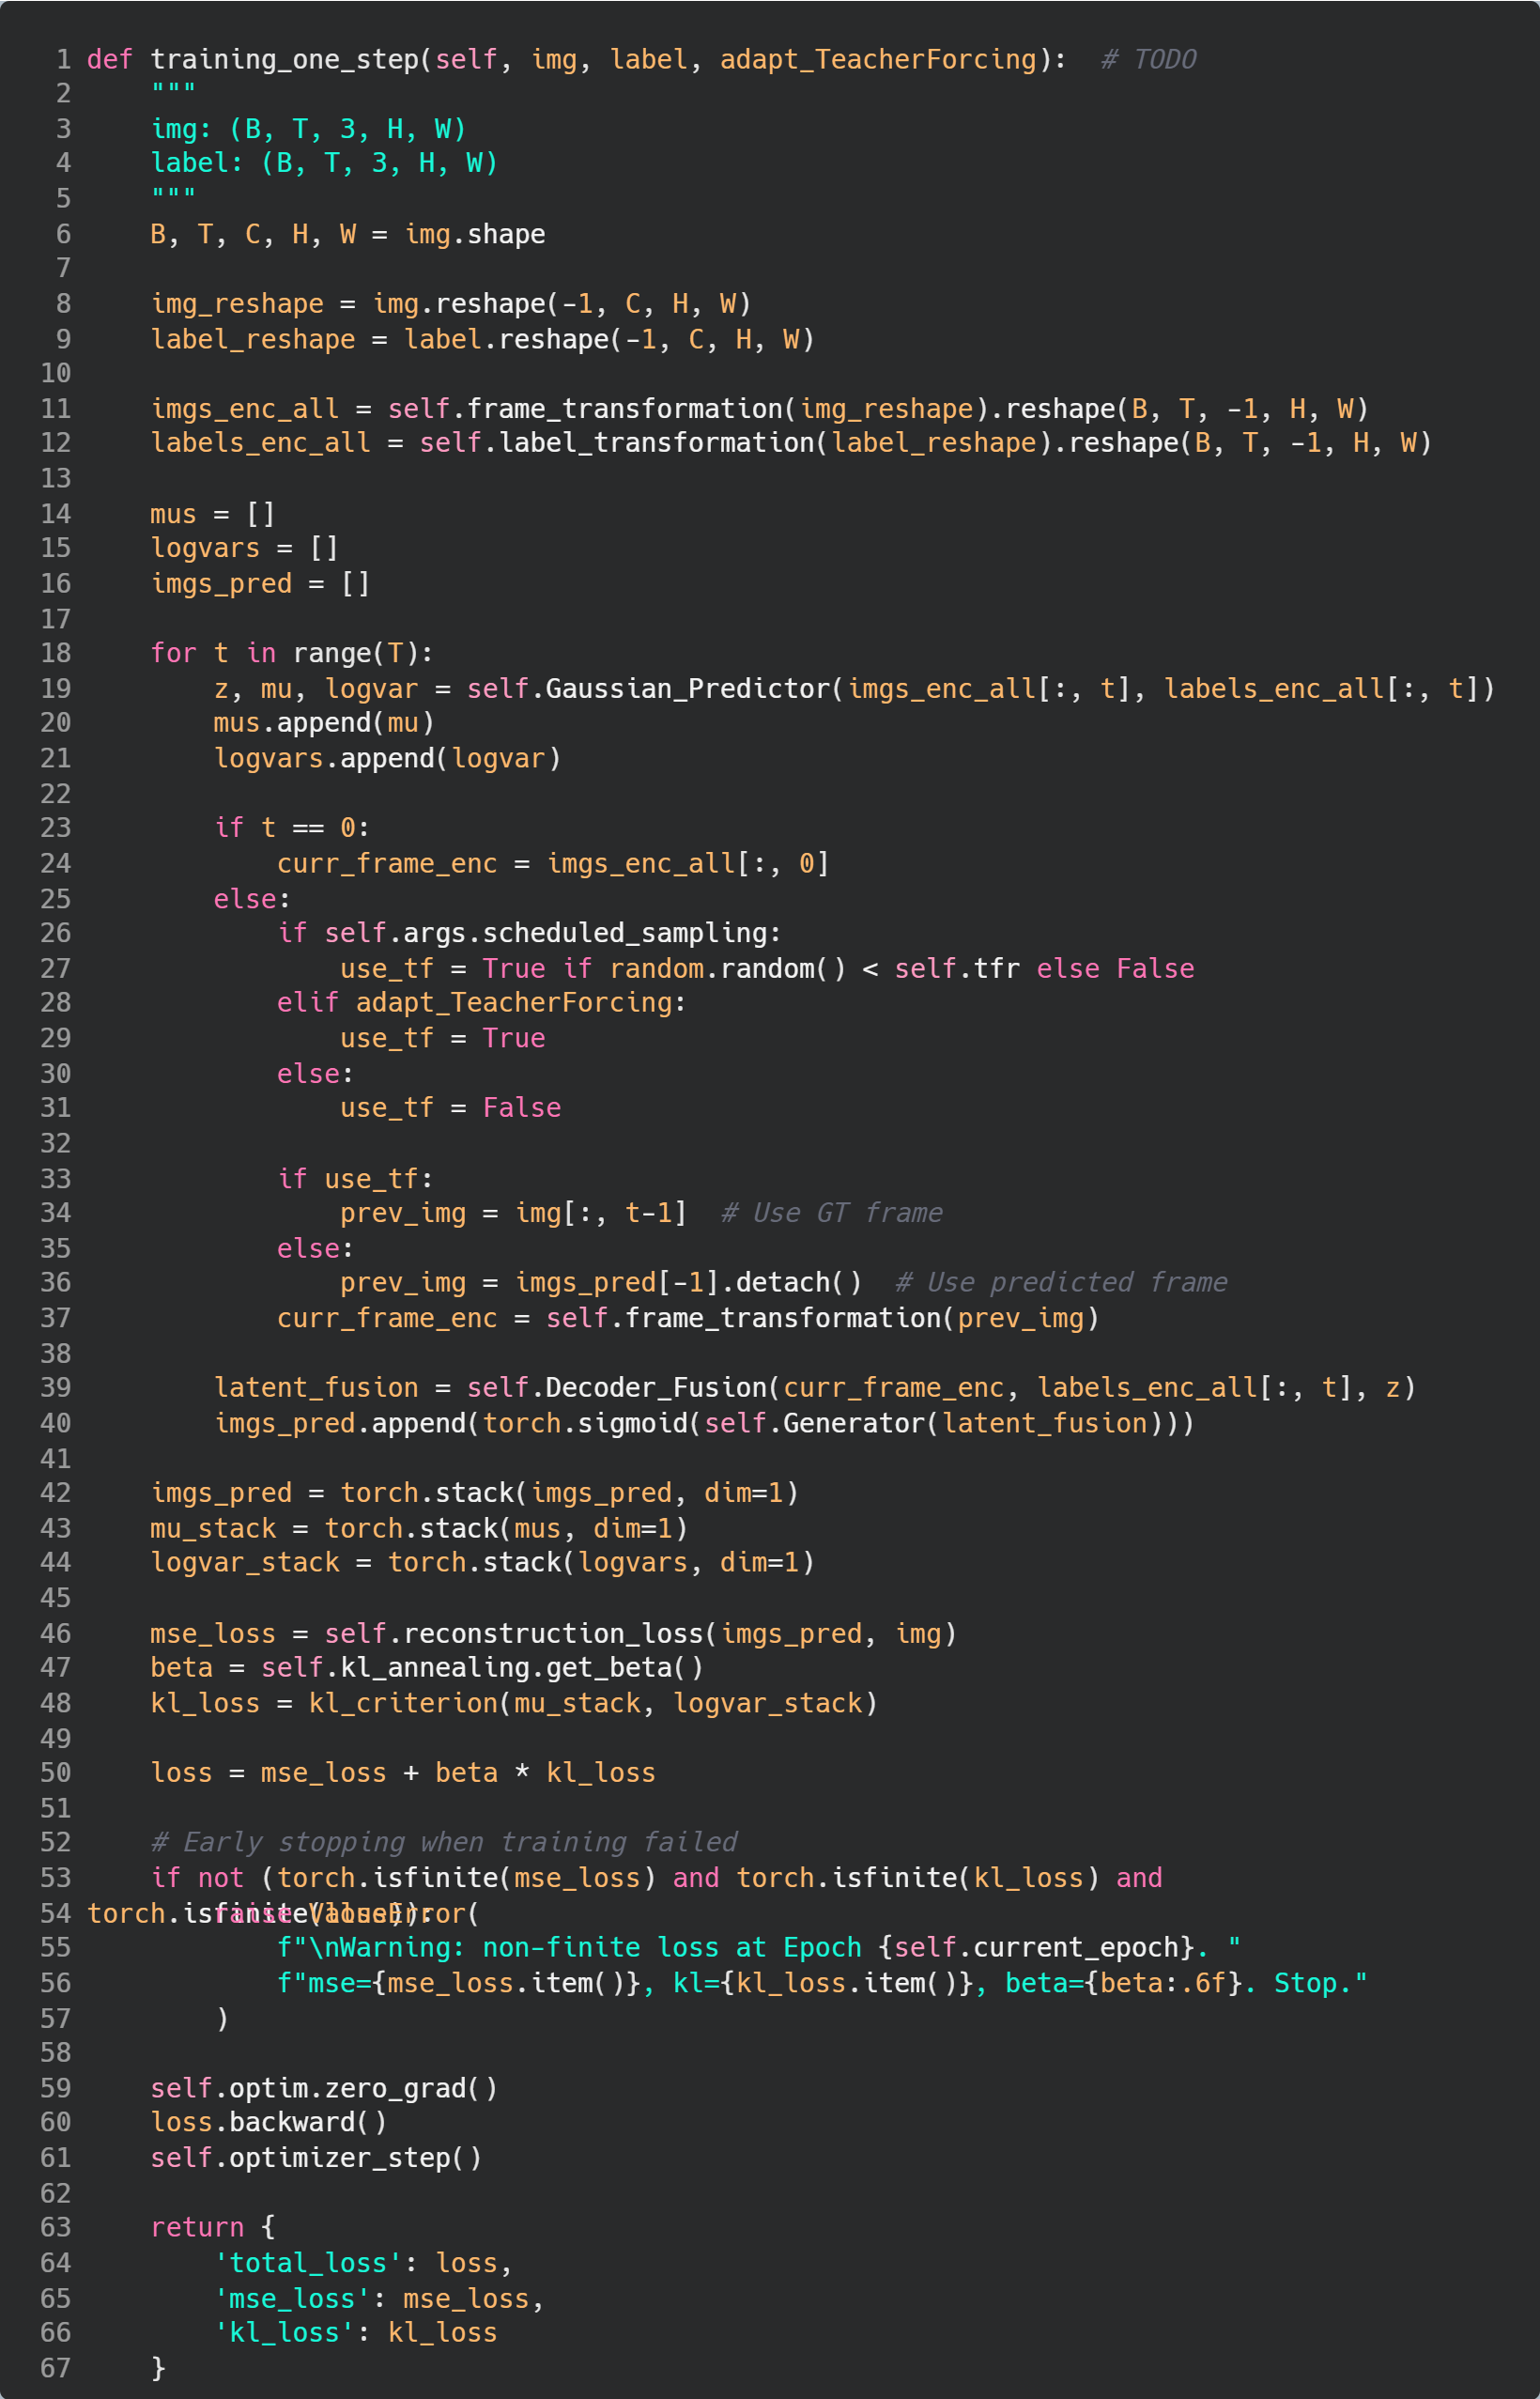
\includegraphics[width=\linewidth]{assets/impl-training_one_step.png}
  \caption{\textbf{Training one step}: encoding, latent prediction, teacher forcing, and decoding.}
  \label{fig:impl_training_one_step}
\end{figure}

After generating the whole predicted sequence, \verb|training_one_step()|
computes a reconstruction term and a KL term:
\begin{equation}
\mathcal{L}=\mathcal{L}_{\text{rec}}+\beta\,\mathcal{L}_{\text{KL}}.
\end{equation}

In practice, $\mathcal{L}_{\text{rec}}$ is MSE (with an optional
tail-weighting that emphasizes later frames), and $\beta$ comes from the KL
annealing scheduler. If the code detects non-finite losses, it raises an error
to stop training early.

In \verb|optimizer_step()|, the code clips gradients and skips the update if it
detects any NaN/Inf in gradients (instead of silently applying a bad step). I
kept these safeguards because some hyper-parameter settings can easily cause
NaNs.

During validation and testing, the model predicts 630 frames per sequence.
Since no ground truth of last frame is available, the model always conditions
on its own previous prediction $\hat{x}_{t-1}$. To reduce variance from a
single latent sample, in testing time, it average multiple latent samples at
each step (Monte Carlo sampling). In my best setting, I use \verb|mc_samples=32|.
The code snippet is in \cref{fig:impl_test}.

\begin{figure}[H]
  \centering
  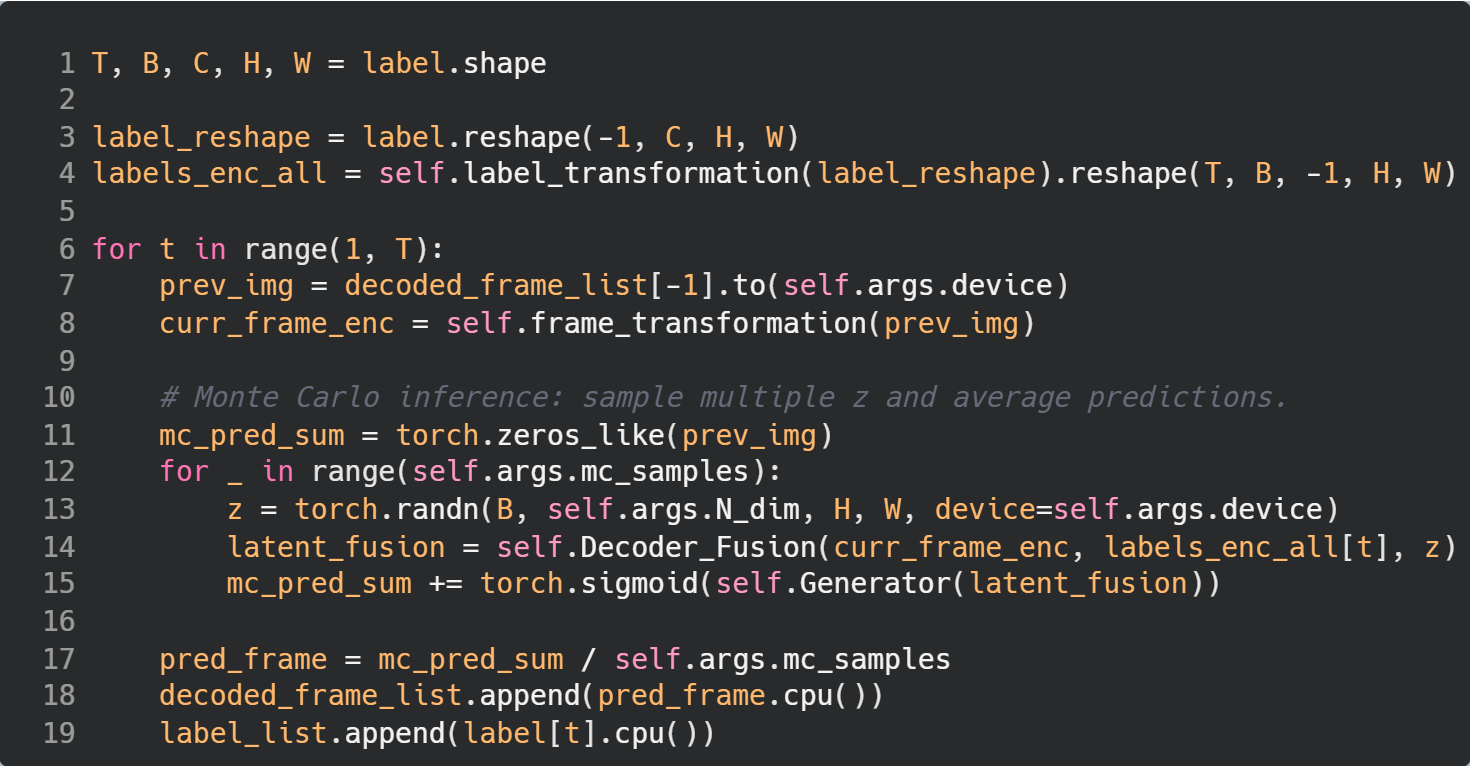
\includegraphics[width=\linewidth]{assets/impl-test.png}
  \caption{Testing logic}
  \label{fig:impl_test}
\end{figure}

\subsection{Reparameterization Trick.}
In \verb|Gaussian_Predictor.reparameterize()|, latent sampling is implemented as
\begin{equation}
\sigma = \exp\left(0.5 \log\sigma^2\right),\ 
\epsilon \sim \mathcal{N}(0, I),\ 
z = \mu + \sigma \odot \epsilon.
\end{equation}
$\mu$ and $\log\sigma^2$ are also clamped for numerical stability,
which is helpful when training becomes unstable.

\begin{figure}[H]
  \centering
  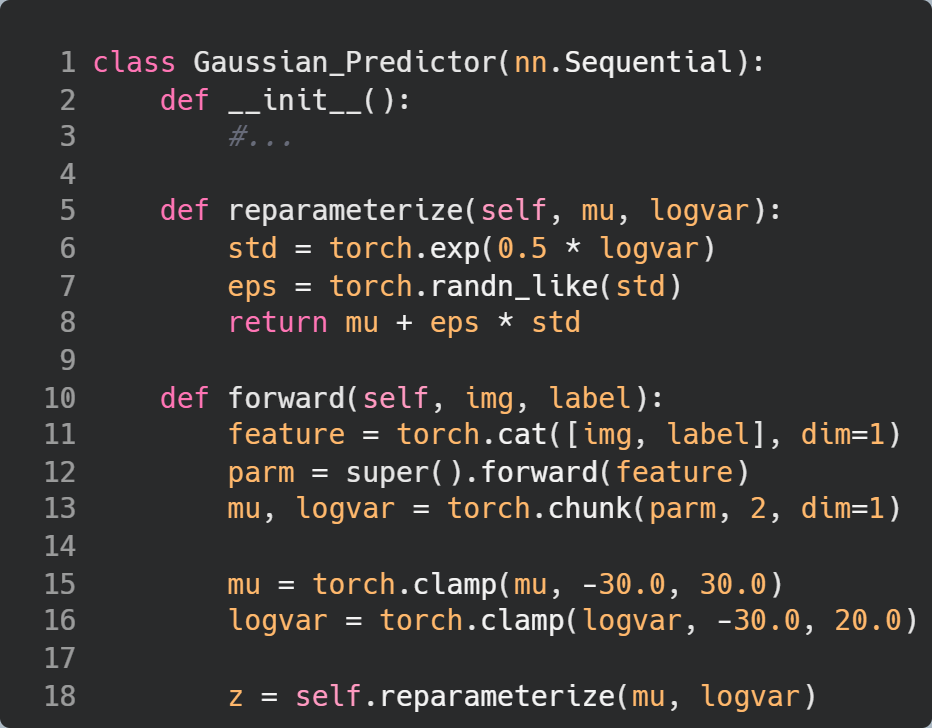
\includegraphics[width=\linewidth]{assets/impl-reparam.png}
  \caption{Reparameterization trick in Gaussian predictor.}
  \label{fig:impl_reparam}
\end{figure}

\subsection{Teacher Forcing Strategy.}
I tried the two teacher forcing strategies:
\begin{itemize}[itemsep=0pt]
  \item \textbf{Per-epoch teacher forcing}: one Bernoulli decision per epoch
  (\verb|adapt_TeacherForcing|); all time steps in that epoch follow the same mode.
  \item \textbf{Scheduled sampling}: one Bernoulli decision per frame
  (enabled by \verb|--scheduled_sampling|).
\end{itemize}
Teacher forcing ratio is decayed by
\begin{equation}
\text{tfr} \leftarrow \max(0, \text{tfr}-\Delta)
\end{equation}
after \verb|current_epoch >= tfr_sde|, where $\Delta$ is
\verb|tfr_d_step|.

\subsection{KL Annealing Ratio}
The \verb|kl_annealing| class supports:
\begin{itemize}[itemsep=0pt]
  \item \textbf{Monotonic}: one linear warm-up from 0 to 1 over the annealing
  portion of training. Here, \verb|kl_anneal_ratio| decides how large this
  warm-up region is, and the same linear ramp is applied once from start to end
  of that region.
  \item \textbf{Cyclical}: the same warm-up idea is repeated in each cycle.
  Within every cycle, \verb|kl_anneal_ratio| still means the fraction of the
  cycle used for ramping up $\beta$, while the remaining part keeps $\beta$ at
  its final value. So compared with monotonic annealing, cyclical annealing is
  basically a repeated warm-up-and-hold schedule.
  \item \textbf{Fixed}: constant $\beta=1$ (no annealing).
\end{itemize}

At initialization, \verb|frange_cycle_linear| is called to calculate
the annealing schedule for the whole training process, and saved in 
\verb|betas|. On each epoch, the current $\beta$ is updated by indexing
into \verb|betas| with the current epoch number.

For robustness, the final beta is lower-bounded by \verb|kl_beta_min|.

\begin{figure}[H]
  \centering
  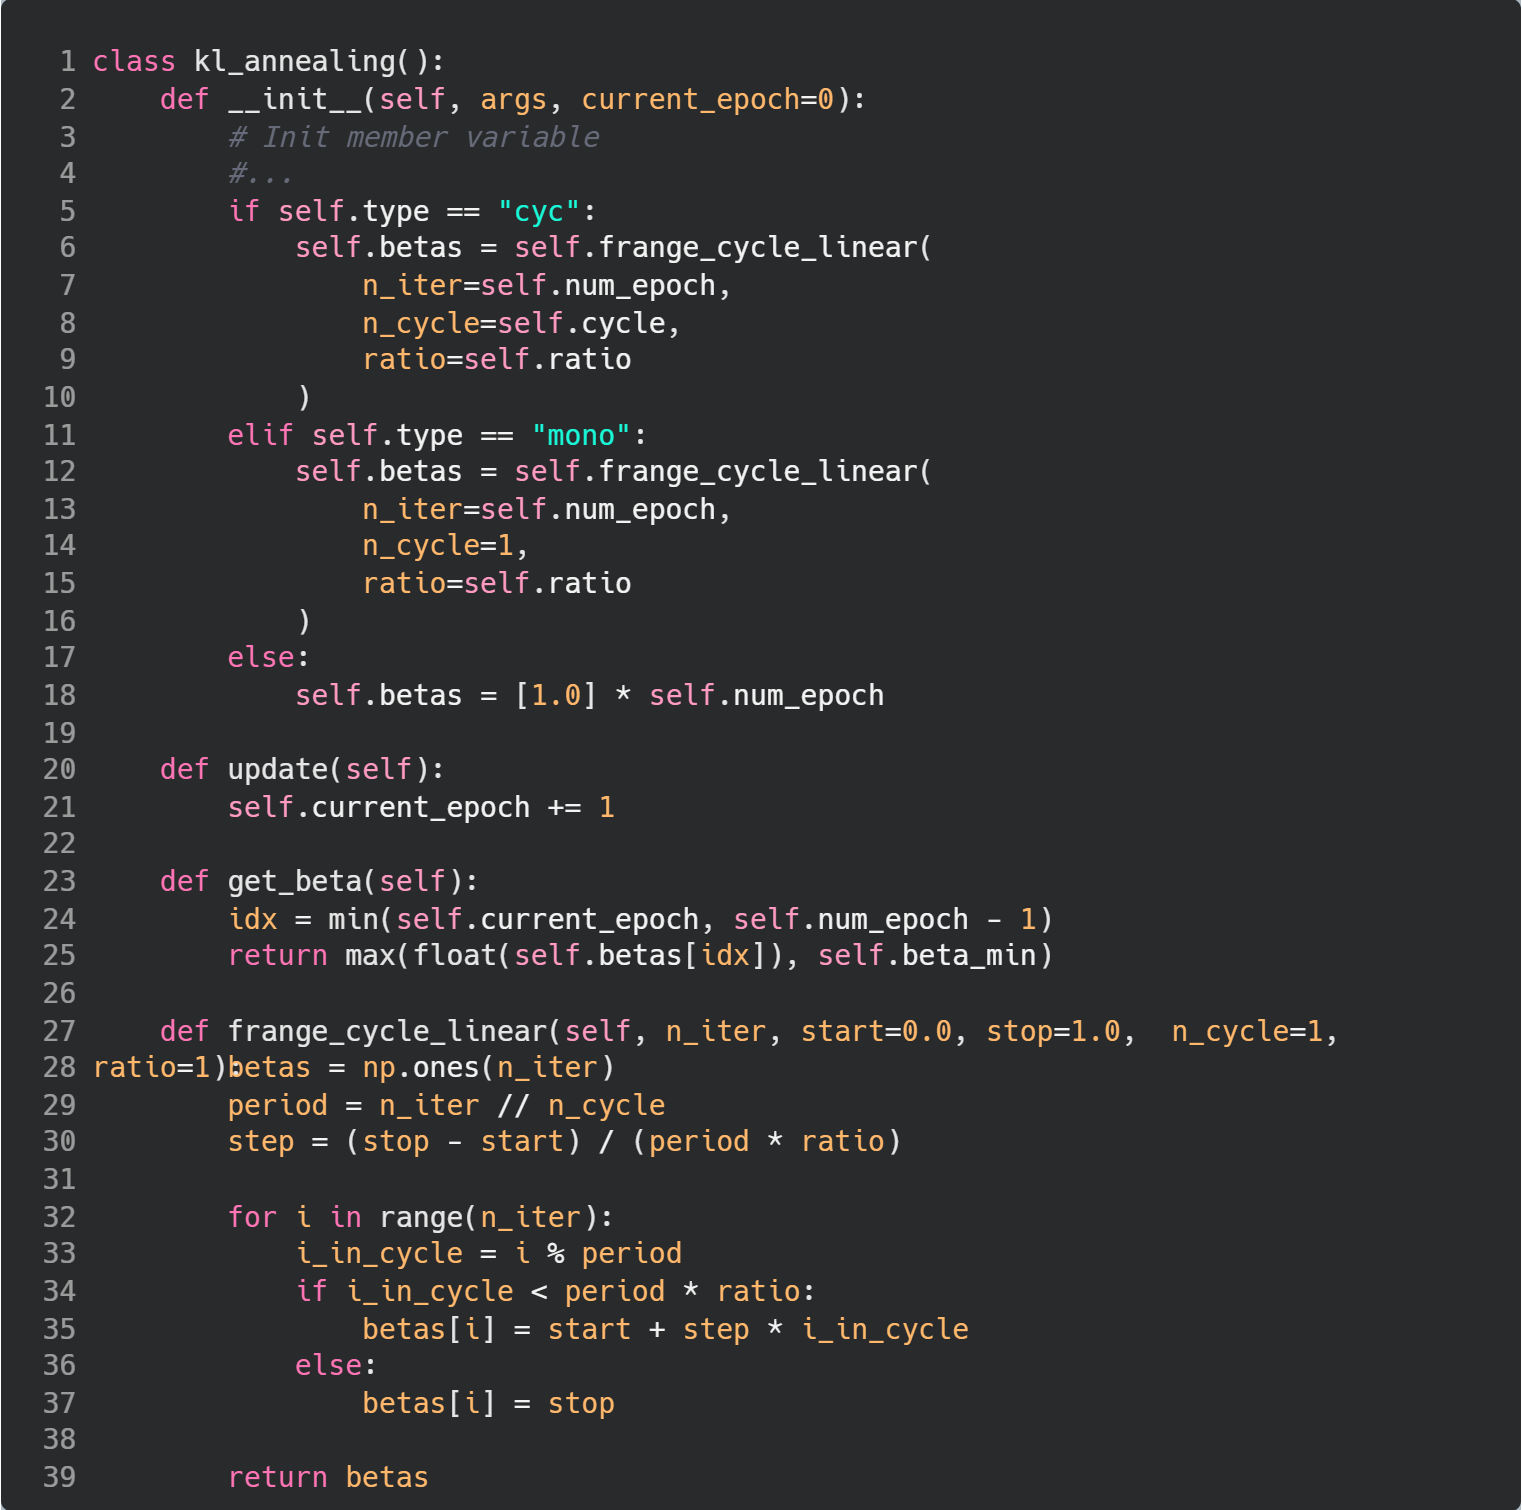
\includegraphics[width=\linewidth]{assets/impl-kl.png}
  \caption{KL annealing schedules.}
  \label{fig:impl_kl}
\end{figure}

\section{Analysis and Discussion}
\label{sec:analysis}

\subsection{Teacher Forcing Ratio and Loss Trend}
\label{sec:tfr}

\Cref{fig:tfr_curve} overlays teacher forcing ratio and training total loss in
the same figure. Since TFR is logged per epoch while loss is logged per step, I
converted loss to an step-aligned horizontal axis for direct comparison. As
tfr decays after the scheduled start epoch, the loss starts to increase and
fluctuate more, which is expected because the model is now conditioning on
its own predictions instead of ground truth. However, after a few epochs of
adaptation, the loss starts to decrease again. This pattern suggests that the
model is successfully transitioning to self-conditioned rollout, and the
initial increase in loss is a sign of the model learning.

\begin{figure}[H]
  \centering
  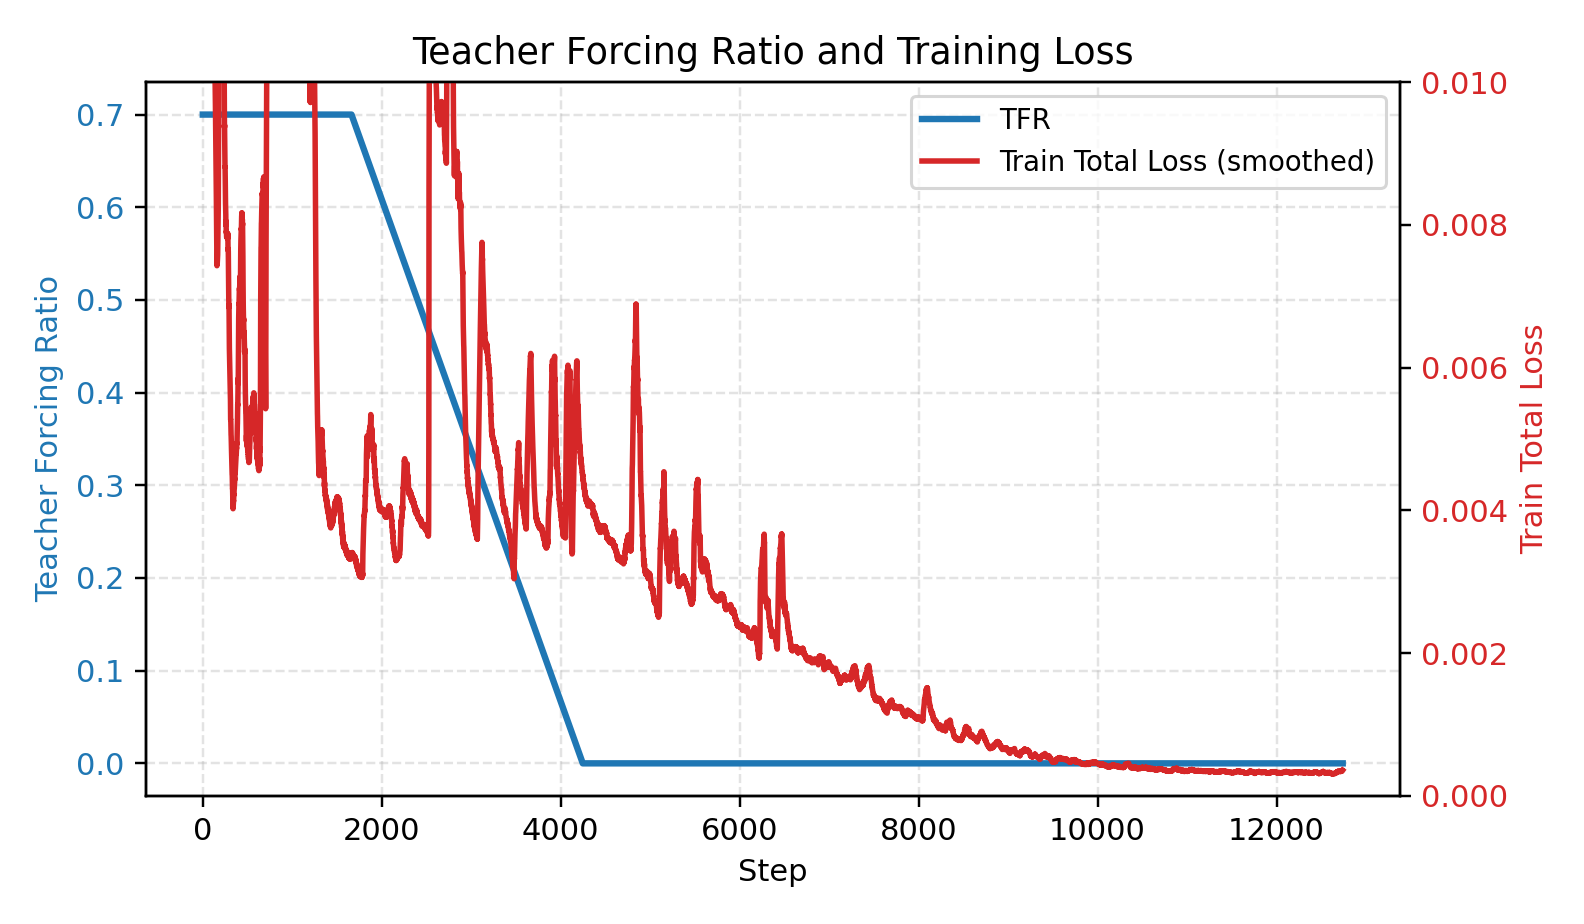
\includegraphics[width=\linewidth]{assets/tfr_curve.png}
  \caption{Teacher forcing ratio and training total loss from the same experiment setting.}
  \label{fig:tfr_curve}
\end{figure}

\Cref{fig:tfr_psnr} also uses the same run and shows how validation PSNR
changes as teacher forcing ratio decreases. Even though PSNR fluctuates early,
it still improves after tfr starts to drop. My interpretation is that once the
model gets used to conditioning on its own predictions, it becomes more robust
for long-horizon rollout.

\begin{figure}[H]
  \centering
  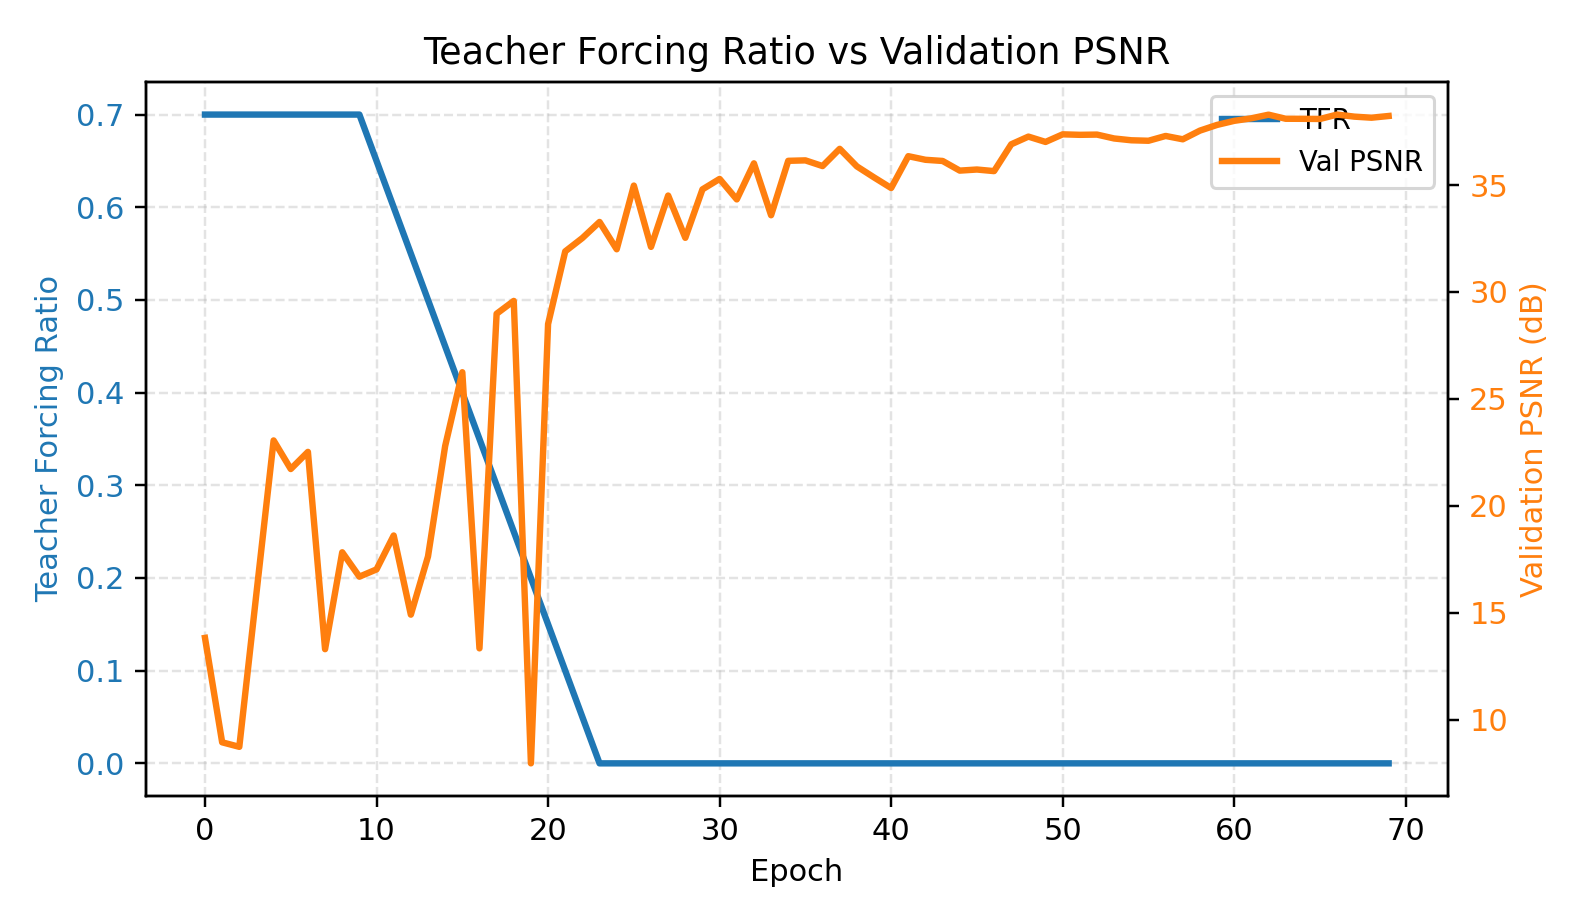
\includegraphics[width=\linewidth]{assets/tfr_vs_psnr.png}
  \caption{Teacher forcing ratio versus validation PSNR from the same experiment setting.}
  \label{fig:tfr_psnr}
\end{figure}

\begin{figure*}[t]
  \centering
  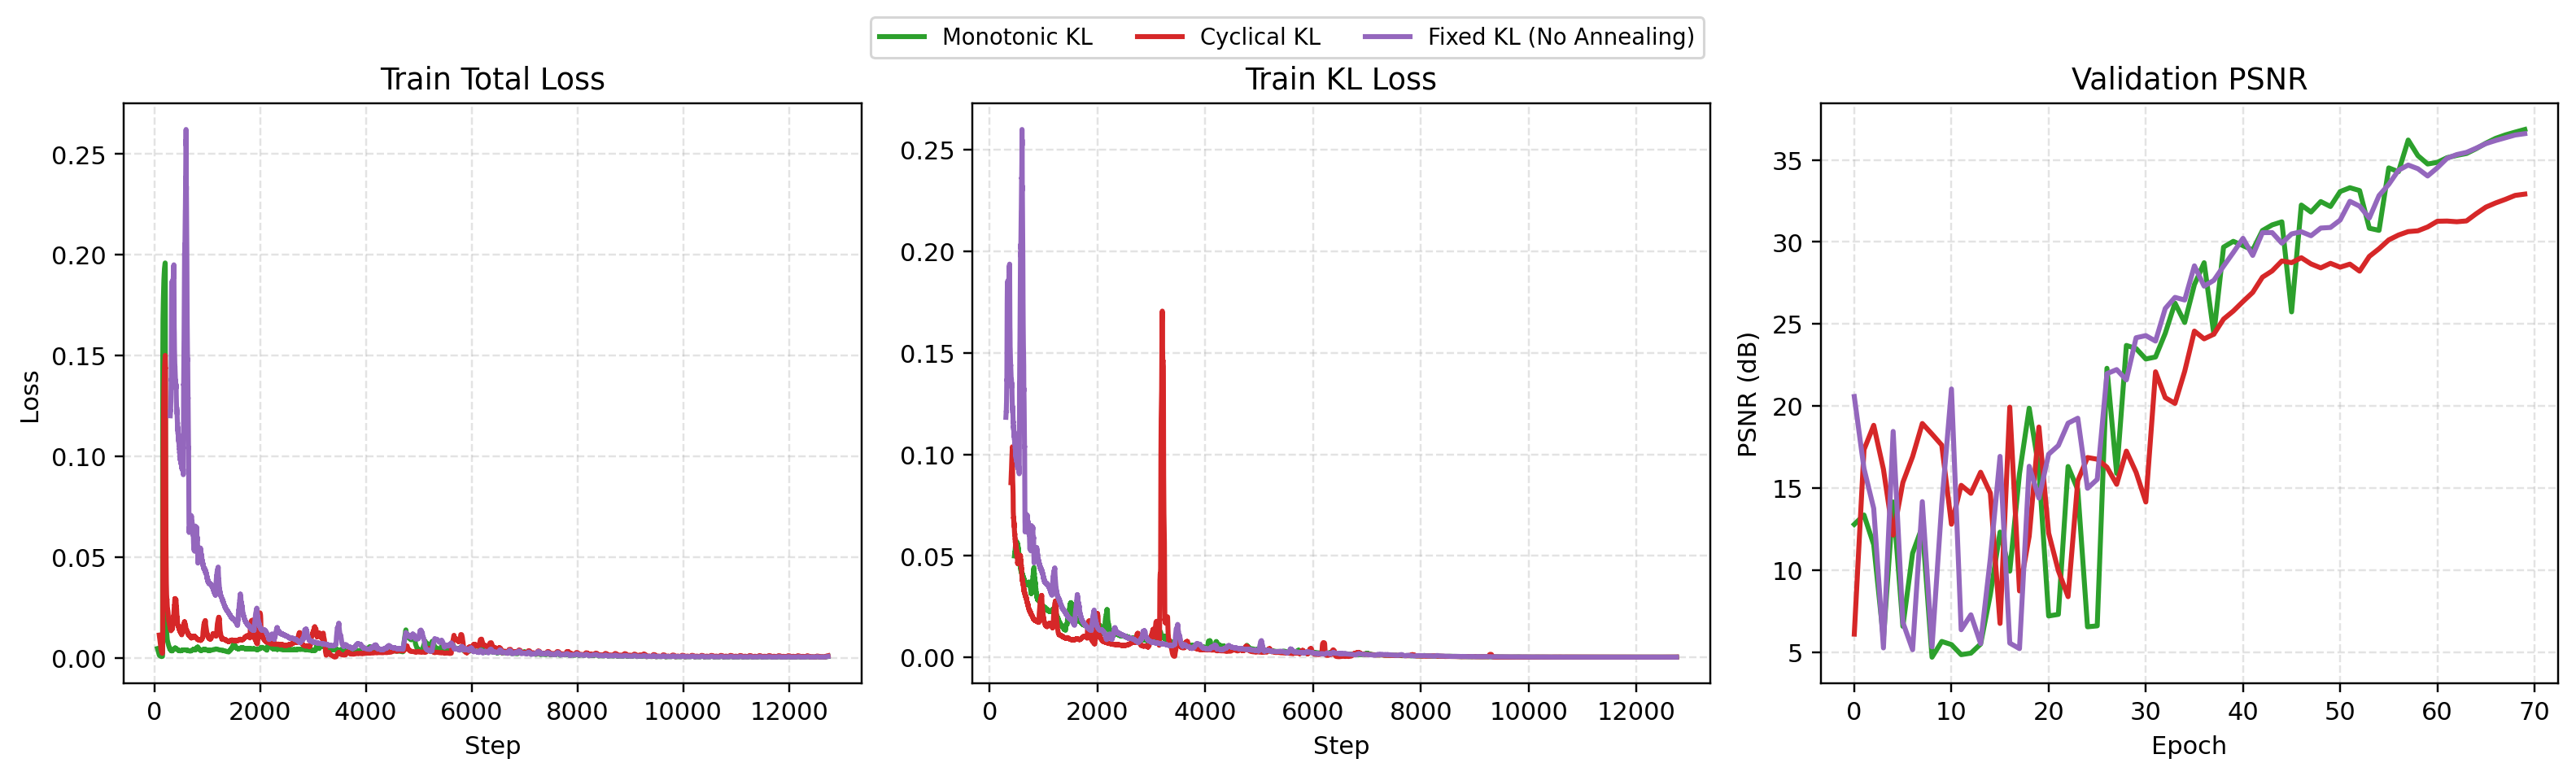
\includegraphics[width=0.95\linewidth]{assets/loss_curve_kl_compare.png}
  \caption{Loss and validation PSNR comparison for monotonic, cyclical, and fixed KL settings.}
  \label{fig:kl_compare}
\end{figure*}

\subsection{Loss Curves Under Different KL Settings}

\Cref{fig:kl_compare} compares three settings:
monotonic KL annealing, cyclical KL annealing, and fixed KL ($\beta=1$,
without annealing).

From my runs, monotonic KL gives the best final validation PSNR and a relatively
stable training process. Cyclical KL can be competitive, but the KL-related
signals oscillate and I found it slightly harder to tune. It needs small 
learning rate to avoid explosion when the restarting happens. From my experiments,
I found that 1e-3 will diverge, 8e-4 will sometimes lead to explosion but can
achieve best PSNR when it works among cyclical settings, and 5e-4 is more
stable but lower best PSNR. And even when successful training is achieved,
the best PSNR is still lower than monotonic KL. Without annealing
($\beta=1$ from the start), suprisingly, is more easy to train than cyclical
KL.

\subsection{PSNR Per Frame on Validation Set}

\Cref{fig:psnr_frame} shows per-frame PSNR from validation dataset during
evaluation. The curve generally decreases with time step, which is expected
because autoregressive prediction accumulates small frame-wise errors. However,
the curve is not strictly monotonic and has some fluctuations. At around frame
400 to 550, the curve shows a more pronounced decline, which may result
from the fact that the motion in that moment is more complex and harder to
predict.

\begin{figure}[H]
  \centering
  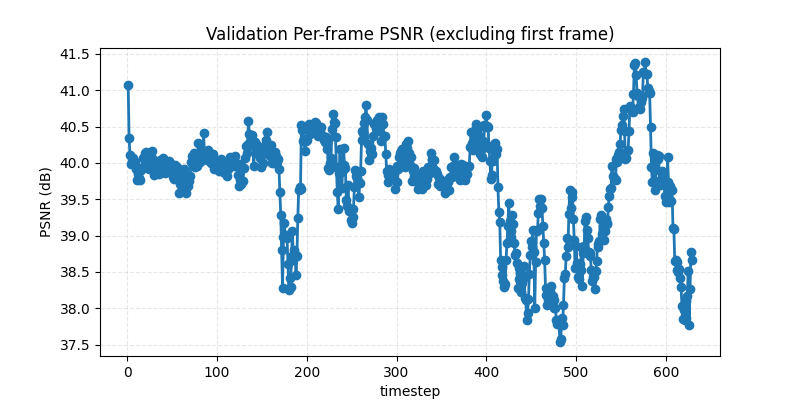
\includegraphics[width=\linewidth]{assets/psnr_per_frame.png}
  \caption{Validation PSNR per frame (from TensorBoard image summary).}
  \label{fig:psnr_frame}
\end{figure}

\subsection{Other Training Strategy Analysis}

\subsection*{Data preparation}

Shuffling the training dataset and using a sliding window to load data
significantly improve the model performance. With the same tfr and KL settings,
the best PSNR I got without shuffling and sliding window is around 37.58, while
adding shuffling can reach around 38.23 and with both tricks can further improve
to around 39.81. I think these strategies increase the diversity of training
samples, which helps the model generalize better.

\subsection*{Analysis of TFR Parameters}

Beyond the single run in \cref{sec:tfr}, I swept over different combinations
of teacher forcing parameters. \Cref{tab:tfr_strategy} compares per-epoch vs.
\ per-frame and different initial \verb|tfr| values. As shown, per-epoch
with \verb|tfr=0.7| gives the best average PSNR. Follow this setting, I
further swept over different decay start epochs (\verb|tfr_sde|) and decay
steps (\verb|tfr_d_step|). The results are summarized in
\cref{tab:tfr_analysis}. It shows that:

\begin{itemize}[itemsep=1pt]
  \item \verb|tfr_sde=10, tfr_d_step=0.05| is the best setting
  \item Larger \verb|tfr_d_step=0.10| often fails (top-right cells)
\end{itemize}

\begin{table}[H]
  \centering
  \begin{tabular}{lcc}
    \toprule
    Configuration & Avg.\ PSNR \\
    \midrule
    Per-epoch (\texttt{tfr=0.7}) & \textbf{35.0} \\
    Per-epoch (\texttt{tfr=1.0}) & 33.1 \\
    Per-frame (\texttt{tfr=0.7}) & 30.8 \\
    Per-frame (\texttt{tfr=1.0}) & 31.6 \\
    \bottomrule
  \end{tabular}
  \caption{\textbf{Effect of TFR strategy and initial ratio.} The max PSNR
    is annotated in bold}
  \label{tab:tfr_strategy}
\end{table}

\begin{table}[H]
  \centering
  \begin{tabular}{ccc}
    \toprule
     & \verb|d_step=0.05| & \verb|d_step=0.10| \\
    \midrule
    \verb|tfr_sde=10| & \textbf{37.56} & failed \\
    \verb|tfr_sde=15| & 36.54 & failed \\
    \verb|tfr_sde=20| & 36.93 & 36.16 \\
    \verb|tfr_sde=25| & 31.86 & 37.16 \\
    \verb|tfr_sde=30| & 35.52 & 36.29 \\
    \bottomrule
  \end{tabular}
  \caption{\textbf{TFR decay parameters: decay start epoch and decay step.}
    The max PSNR is annotated in bold.}
  \label{tab:tfr_analysis}
\end{table}

\subsection*{Monte Carlo Averaging at Inference}

As mentioned in \cref{sec:training_testing}, I used multiple latent samples
at each step during inference to reduce variance in predictions. In my
experiments, I found that increasing the number of Monte Carlo samples from
1 to 32 can give a slight improvement in PSNR.

\section{Conclusion}

In this lab, I learned that the model quality is very sensitive to training
curriculum. In my experiments, the best result comes from using shuffled
training windows, stride 8, monotonic KL annealing, and the teacher forcing
schedule \verb|tfr=0.7, tfr_sde=10, tfr_d_step=0.05|. For the final
sampling stage, \verb|mc_samples=32| gives a noticeable improvement by
reducing sampling variance.

Overall, teacher forcing decay and KL annealing help the model transition from
easy (ground-truth conditioned) training to harder (self-conditioned) rollout.
However, I still see a clear PSNR drop in later frames, so long-horizon drift is
still the main limitation of my current implementation.

% %%%%%%%%% REFERENCES %%%%%%%%%
% {\small
% \bibliographystyle{ieee_fullname}
% \bibliography{egbib}
% }

\end{document}